
\documentclass[10pt]{report}
%Packages
\usepackage{multirow}
\usepackage{graphicx}
\usepackage[utf8x]{inputenc}
\usepackage[T1]{fontenc}
\usepackage{aeguill}
\usepackage{amssymb}
\usepackage[french]{babel}
\usepackage{float}
\usepackage{fichetd}
\usepackage{mathenv}
\usepackage{tikz}
\usepackage[a4paper,pdftex=true]{geometry}
\usepackage{fancyvrb}

%Preamble

\input Cours/cqlsInclude
\input Cours/testInclude


\rightmargin -2cm
\leftmargin -1cm
\topmargin -2cm
\textheight 25cm

\newcommand{\redabr}{\textit{(rédaction abrégée) }}
\newcommand{\redstd}{\textit{(rédaction standard) }}

\setcounter{chapter}{6}
%Styles

%Title

\begin{document}




\chapter{Exos généraux}

\begin{exercice} (second tour des élections présidentielles - Mai 2002)

Un professeur de statistiques souhaite utiliser le r{\'e}sultat du premier tour des {\'e}lections pr{\'e}sidentielles 2002 afin de mener {\`a} bien un exercice {\bf p{\'e}dagogique} avec ses $m=100$ {\'e}tudiants. L'id{\'e}e est la suivante : chaque {\'e}tudiant doit interroger 200 {\'e}lecteurs compl{\`e}tement au hasard (nous supposerons ceci possible et r{\'e}alisable) et leur demander s'ils se sont abstenus ou pas (nous supposerons {\'e}galement que chacun des {\'e}lecteurs interrog{\'e}s d{\'e}clare la v{\'e}rit{\'e}). La consigne de l'exercice est la suivante : essayez au vu de votre {\'e}chantillon de taille $n=200$ de montrer qu'au seuil de 5\%, le taux d'abstention est sup{\'e}rieur {\`a} 28.4\%.\\

Nous noterons $p^{Ab}$ le taux d'abstention (que l'on a suppos{\'e} inconnu) du premier tour, et ${\bf y}_{[1]}$,  l${\bf y}_{[2]}$, $\ldots, {\bf y}_{[100]}$,  les $m=100$ {\'e}chantillons de taille 200 obtenus par chacun des {\'e}tudiants. \\

\begin{enumerate}
\item Un des {\'e}tudiants (le 51{\`e}me) a obtenu une estimation $\Est{p^{Ab}}{y_{[51]}}=29\%$. Parvient-il au seuil de 5\% {\`a} montrer que $p^{Ab}$ est sup{\'e}rieur {\`a} 28.4\%?

\IndicR
\begin{Verbatim}[frame=leftline,fontfamily=tt,fontshape=n,numbers=left]
> # deltaEst51.H0 <- (instruction R à fournir dans la rédaction)
> deltaEst51.H0
[1] 0.1881701
\end{Verbatim}





\item On fournit les sorties \verb+R+ des 100 estimations $\Est{p^{Ab}}{y_{[1]}}$, $\Est{p^{Ab}}{y_{[2]}}$, $\ldots, \Est{p^{Ab}}{y_{[100]}}$ (vecteur \verb+pEst+) du taux d'abstention (rang{\'e}es par ordre croissant) obtenues par chacun des {\'e}tudiants, ainsi que les valeurs respectives $\Est{\delta_{p^{Ab},28.4\%}}{y_{[1]}}, \Est{\delta_{p^{Ab},28.4\%}}{y_{[2]}},\ldots,\Est{\delta_{p^{Ab},28.4\%}}{y_{[100]}}$  (vecteur \verb+est.delta+). Sans aucun calcul suppl{\'e}mentaire, combien d'{\'e}tudiants parviennent au vu de leur propre {\'e}chantillon {\`a} conclure au seuil de 5\%  $p$ est sup{\'e}rieur {\`a} 28.4\%?



\IndicR
\begin{Verbatim}[frame=leftline,fontfamily=tt,fontshape=n,numbers=left]
> pEst
  [1] 0.215 0.220 0.220 0.230 0.240 0.240 0.240 0.245 0.245 0.245 0.245 0.250
 [13] 0.255 0.255 0.260 0.260 0.265 0.265 0.265 0.265 0.265 0.270 0.270 0.270
 [25] 0.275 0.275 0.275 0.275 0.275 0.275 0.275 0.280 0.280 0.280 0.280 0.280
 [37] 0.280 0.280 0.280 0.285 0.285 0.285 0.285 0.285 0.285 0.290 0.290 0.290
 [49] 0.290 0.290 0.290 0.290 0.290 0.290 0.290 0.290 0.290 0.295 0.295 0.295
 [61] 0.295 0.295 0.295 0.295 0.295 0.300 0.300 0.305 0.305 0.305 0.305 0.305
 [73] 0.305 0.305 0.310 0.315 0.315 0.315 0.315 0.320 0.320 0.320 0.320 0.325
 [85] 0.325 0.325 0.325 0.325 0.330 0.330 0.335 0.335 0.335 0.335 0.335 0.335
 [97] 0.345 0.345 0.350 0.365
> deltaEst.H0<-(pEst-.284)/sqrt(.284*(1-.284)/200)
> deltaEst.H0
  [1] -2.16395591 -2.00714751 -2.00714751 -1.69353071 -1.37991391 -1.37991391
  [7] -1.37991391 -1.22310551 -1.22310551 -1.22310551 -1.22310551 -1.06629711
 [13] -0.90948871 -0.90948871 -0.75268032 -0.75268032 -0.59587192 -0.59587192
 [19] -0.59587192 -0.59587192 -0.59587192 -0.43906352 -0.43906352 -0.43906352
 [25] -0.28225512 -0.28225512 -0.28225512 -0.28225512 -0.28225512 -0.28225512
 [31] -0.28225512 -0.12544672 -0.12544672 -0.12544672 -0.12544672 -0.12544672
 [37] -0.12544672 -0.12544672 -0.12544672  0.03136168  0.03136168  0.03136168
 [43]  0.03136168  0.03136168  0.03136168  0.18817008  0.18817008  0.18817008
 [49]  0.18817008  0.18817008  0.18817008  0.18817008  0.18817008  0.18817008
 [55]  0.18817008  0.18817008  0.18817008  0.34497848  0.34497848  0.34497848
 [61]  0.34497848  0.34497848  0.34497848  0.34497848  0.34497848  0.50178688
 [67]  0.50178688  0.65859528  0.65859528  0.65859528  0.65859528  0.65859528
 [73]  0.65859528  0.65859528  0.81540368  0.97221207  0.97221207  0.97221207
 [79]  0.97221207  1.12902047  1.12902047  1.12902047  1.12902047  1.28582887
 [85]  1.28582887  1.28582887  1.28582887  1.28582887  1.44263727  1.44263727
 [91]  1.59944567  1.59944567  1.59944567  1.59944567  1.59944567  1.59944567
 [97]  1.91306247  1.91306247  2.06987087  2.54029607
\end{Verbatim}





\item Tout le monde sait que le taux d'abstention au premier tour des {\'e}lections pr{\'e}sidentielles 2002 a {\'e}t{\'e} de 28.40\%~ : on est donc dans la ``pire des situations'' (i.e. sous $H_0$). Etes-vous {\'e}tonn{\'e} du r{\'e}sultat de la question 2. (justifiez votre r{\'e}ponse). 



\item La variable \texttt{R}, \texttt{IC}, correspond à un intervalle de confiance de $p$ (au niveau 95\%) obtenu pour le 51{\`e}me {\'e}tudiant, pour lequel $\Est{p^{Ab}}{y_{[51]}}=29\%$. Quelle est l'instrcution qui a permis de l'obtenir~?

\noindent {\bf Indications} : 

\begin{Verbatim}[frame=leftline,fontfamily=tt,fontshape=n,numbers=left]
> # IC <- (instruction R à fournir dans la rédaction)
> IC
[1] 0.2271129 0.3528871
\end{Verbatim}




\item a) Si l'on construisait pour chacune des estimations du taux d'abstention un intervalle de confiance au niveau de confiance de 95\%, combien de ces intervalles (en proportion, approximativement) contiendraient la vraie valeur $p^{Ab}=28.4\%$.



b) On observe que 96 {\'e}tudiants obtiennent un intervalle de confiance contenant la valeur $p^{Ab}=28.4\%$. Qu'en pensez-vous? 




\end{enumerate}
\end{exercice}

\begin{exercice} (confrontation entre deux candidats - mai 2004) 

Deux candidats, notés C1 et C2, se confrontent au second tour des élections présidentielles. On notera $p^{C1}$ et $p^{C2}$ ($=1-p^{C1}$) les proportions d'intention de votes pour chacun des deux candidats. Un professeur de statistiques propose à ses $m=200$ étudiants un exercice pédagogique afin d'appréhender les erreurs de décision d'un test d'hypothèses via une approche expérimentale. La consigne est la suivante~: chacun des 200 étudiants doit interroger $n=30$ individus et proposer une estimation de $p^{C1}$.

\begin{enumerate}
\item Uniquement à partir du paramètre $p^{C1}$, décrire l'hypothèse de test $H_1$ (assertion d'intérêt) conduisant à l'élection du candidat C1 puis celle conduisant à l'élection de C2.

\item On fournit ci-dessous les $m=200$ estimations de $p^{C1}$ notées $\Est{p^{C1}}{y_{[j]}}$ ($j=1,\ldots,m$) et stockées et rangées dans l'ordre croissant  dans le vecteur \texttt{pEst} ainsi que les  p$-$valeurs respectives du test $H_1: p^{C1}>50\%$. Parmi les  200 étudiants combien parviennent à dire que l'un des deux candidats (en précisant lequel) sera élu au seuil de 5\%~? (justifiez votre réponse)


\begin{Verbatim}[frame=leftline,fontfamily=tt,fontshape=n,numbers=left]
> pEst
  [1] 0.2666667 0.3000000 0.3000000 0.3333333 0.3333333 0.3666667 0.3666667
  [8] 0.3666667 0.3666667 0.4000000 0.4000000 0.4000000 0.4000000 0.4000000
...
[141] 0.6000000 0.6000000 0.6000000 0.6000000 0.6000000 0.6000000 0.6000000
[148] 0.6000000 0.6000000 0.6000000 0.6000000 0.6000000 0.6333333 0.6333333
[155] 0.6333333 0.6333333 0.6333333 0.6333333 0.6333333 0.6333333 0.6333333
[162] 0.6333333 0.6333333 0.6333333 0.6333333 0.6333333 0.6666667 0.6666667
[169] 0.6666667 0.6666667 0.6666667 0.6666667 0.6666667 0.6666667 0.6666667
[176] 0.6666667 0.6666667 0.6666667 0.6666667 0.6666667 0.6666667 0.6666667
[183] 0.6666667 0.6666667 0.6666667 0.7000000 0.7000000 0.7000000 0.7000000
[190] 0.7000000 0.7000000 0.7000000 0.7000000 0.7333333 0.7333333 0.7333333
[197] 0.7666667 0.7666667 0.7666667 0.7666667
> 1-pnorm(pEst,0.5,sqrt(0.5*0.5/30))
  [1] 0.994706431 0.985770132 0.985770132 0.966055423 0.966055423 0.927936483
  [7] 0.927936483 0.927936483 0.927936483 0.863339161 0.863339161 0.863339161
...
[151] 0.136660839 0.136660839 0.072063517 0.072063517 0.072063517 0.072063517
[157] 0.072063517 0.072063517 0.072063517 0.072063517 0.072063517 0.072063517
[163] 0.072063517 0.072063517 0.072063517 0.072063517 0.033944577 0.033944577
[169] 0.033944577 0.033944577 0.033944577 0.033944577 0.033944577 0.033944577
[175] 0.033944577 0.033944577 0.033944577 0.033944577 0.033944577 0.033944577
[181] 0.033944577 0.033944577 0.033944577 0.033944577 0.033944577 0.014229868
[187] 0.014229868 0.014229868 0.014229868 0.014229868 0.014229868 0.014229868
[193] 0.014229868 0.005293569 0.005293569 0.005293569 0.001743502 0.001743502
[199] 0.001743502 0.001743502
\end{Verbatim}



Le second tour des élections s'est déroulé, et nous pouvons observer que le candidat C1 a été élu avec une proportion d'intentions de vote $p^{C1}=55\%$. \\

\item a) Quelle était la nature du risque d'erreur de décision (du test cherchant à montrer que C1 sera élu) compte tenu de la vraie situation~? \\
b) Au vu des 200 p$-$valeurs précédentes, donnez l'ordre de grandeur de ce risque~?\\
c) A quoi pouvait-on s'attendre au vu des instructions ci-dessous~? Autrement dit, si le nombre d'étudiants avait été infini combien en proportion auraient décidé l'élection de C1~?


\begin{Verbatim}[frame=leftline,fontfamily=tt,fontshape=n,numbers=left]
> pnorm(qnorm(0.95,0.5,sqrt(0.5*0.5/30)),0.55,sqrt(0.55*0.45/30))
[1] 0.8649122
> pnorm(qnorm(0.05,0.5,sqrt(0.5*0.5/30)),0.55,sqrt(0.55*0.45/30))
[1] 0.01377547
> 1-pnorm(qnorm(0.05,0.5,sqrt(0.5*0.5/30)),0.45,sqrt(0.55*0.45/30))
[1] 0.8649122
> 1-pnorm(qnorm(0.95,0.5,sqrt(0.5*0.5/30)),0.45,sqrt(0.55*0.45/30))
[1] 0.01377547
\end{Verbatim}


\item Mêmes questions pour le candidat C2 (i.e. remplacer C1 par C2 dans les questions a), b) et c) précédentes.



\item 
a) Donner l'instruction \texttt{R} permettant d'évaluer l' intervalle de confiance du paramètre $p^{C1}$ au niveau de confiance 95\% pour le 11-éme étudiant (pour lequel $\Est{p^{C1}}{y_{[11]}}=40\%$). \\
b) On fournit ci-dessous les onze premiers et derniers intervalles de confiance des 200 étudiants. Parmi les 200 étudiants combien en proportion ont un intervalle de confiance contenant le paramètre $p^{C1}$. Le 11-ème étudiant a-t-il eu de la chance~?\\
c) Comparez le résultat obtenu en b) avec celui que l'on pourrait obtenir si l'on disposait d'une infinité d'étudiants~?

\begin{Verbatim}[frame=leftline,fontfamily=tt,fontshape=n,numbers=left]
pInf      pSup
1   0.1084244 0.4249090
2   0.1360176 0.4639824
3   0.1360176 0.4639824
4   0.1646465 0.5020202
5   0.1646465 0.5020202
6   0.1942261 0.5391072
7   0.1942261 0.5391072
8   0.1942261 0.5391072
9   0.1942261 0.5391072
10  0.2246955 0.5753045
11  0.2246955 0.5753045
...
189 0.5360176 0.8639824
190 0.5360176 0.8639824
191 0.5360176 0.8639824
192 0.5360176 0.8639824
193 0.5360176 0.8639824
194 0.5750910 0.8915756
195 0.5750910 0.8915756
196 0.5750910 0.8915756
197 0.6153178 0.9180155
198 0.6153178 0.9180155
199 0.6153178 0.9180155
200 0.6153178 0.9180155
\end{Verbatim}


\end{enumerate}
\end{exercice}

\begin{exercice}

Dans un certain pays, trois candidats se présentent aux élections présidentielles. Au premier tour, le candidat ayant eu le moins d'intentions de vote sera éliminé. Pour s'assurer qu'il sera au tour suivant, l'un des candidats comprend donc qu'il lui suffit d'obtenir plus d'un tiers des intentions de vote. Il interroge $n=100$ électeurs, sur cet échantillon, 60 s'engagent à voter pour lui.

\begin{enumerate}
\item Peut-on penser que ce candidat sera au second tour~?

\IndicR
\begin{Verbatim}[frame=leftline,fontfamily=tt,fontshape=n,numbers=left]
> (60/100-1/3)/sqrt((1/3*(1-1/3))/100)
[1] 5.656854
\end{Verbatim}





\item Ne peut-on pas affirmer autre chose au vu de l'instruction ci-dessous (\textit{Indication: rédaction abrégée})~?

\IndicR
\begin{Verbatim}[frame=leftline,fontfamily=tt,fontshape=n,numbers=left]
> (60/100-.5)/sqrt(.5*.5/100)
[1] 2
\end{Verbatim}




\item Le candidat construit un intervalle de confiance de la proportion d'intentions de vote en sa faveur au niveau de confiance 95\%. Il obtient l'intervalle [50.4\%,69.6\%]. Donnez l'instruction \texttt{R} permettant d'obtenir cet intervalle de confiance.


 


\item Comment interprétez-vous cet intervalle de confiance~?





\end{enumerate}
\end{exercice}

\begin{exercice}[Assemblée générale étudiante]~ 

Durant le mouvement de grève anti-cpe, un étudiant (fan de statistiques) qui se trouve à l'une des assemblées générales, est impatient de connaître le résultat des votes relatif au blocage ou à la reprise des cours. Pour tenter d'avoir une idée sur la question, il décide d'interroger au hasard 51 étudiants parmi les participants de l'assemblée générale. Sur 51 étudiants, 35 se sont prononcés pour le blocage. 

\begin{enumerate}
\item 
A partir de cette estimation, il construit un intervalle de confiance de la proportion des bloqueurs au niveau de confiance 95\%. Assez surdoué en calcul mental, il obtient l'intervalle [58.1\%,83.1\%]. Supposons que vous soyez moins doué en calcul mental, mais que vous disposez d'un portable et du logiciel \texttt{R}. Donnez l'instruction \texttt{R} permettant d'obtenir cet intervalle de confiance.


 


\item 
Comment interprétez-vous cet intervalle de confiance~?





\item  
A la vue de l'intervalle de confiance, l'étudiant pense que les cours ne vont pas reprendre et vous qu'en pensez-vous~?





\item  
L'étudiant sait pourtant que pour répondre correctement à cette question, il faut réaliser un test d'hypothèses. Il met en place un test d'hypothèses permettant de savoir si le blocage va être reconduit. En prenant un risque d'erreur de 5\%, rédigez ce test sous la forme standard.

\IndicR
\begin{Verbatim}[frame=leftline,fontfamily=tt,fontshape=n,numbers=left]
> # deltaEst.H0 <- (instruction R à fournir dans la rédaction)
> deltaEst.H0
[1] 2.660532
\end{Verbatim}





\end{enumerate}


\end{exercice}

\begin{exercice} (Premier tour élections présidentielles de 2007)
${ }$

\noindent \underline{Partie~I~: finalisation de la décision}

1)  
Plaçons-nous une semaine avant le premier tour des élections présidentielles. A cette date, on crée un échantillon de taille $n=1000$ pour savoir si la proportion d'électeurs indécis est strictement supérieure à 30\%. Au vu des données stockées dans le vecteur \texttt{yI1} en \texttt{R}, peut-on affirmer \redabr cette assertion au seuil de 5\%~? 

\IndicR
\begin{Verbatim}[frame=leftline,fontfamily=tt,fontshape=n,numbers=left]
> yI1
   [1] 0 1 0 0 1 1 1 0 0 1 0 0 0 1 0 1 0 0 0 1 0 0 1 1 0 1 1 1 0 0 1 1 0 1 1 0 1
  [38] 0 0 0 0 0 0 0 1 1 0 0 0 0 0 0 0 1 0 1 1 0 0 0 1 1 1 0 0 0 0 1 1 0 1 1 1 0
...
[1000] 1
> mean(yI1)
[1] 0.372
> # deltaEst.H0 <- (instruction R à fournir dans la rédaction)
> pnorm(deltaEst.H0)
[1] 0.9999997
\end{Verbatim}





2) 
La veille du scrutin, on interroge $n=500$ {\bf nouveaux} individus, les données étant stockées dans vecteur \texttt{yI2} en \texttt{R}. Peut-on plutôt penser \redstd que la proportion d'électeurs indécis à la veille du scrutin est plus de deux fois plus petite que celle de la semaine précédente~?  \\
\underline{Indication~:} comme une proportion est aussi une moyenne (de 0 et de 1), pour cette question, on pourra aussi noter $\mu^{I1}$ et $\mu^{I2}$ les proportions d'électeurs indécis une semaine avant (i.e. $p^{I1}$) et la veille du scrutin (i.e. $p^{I2}$).


\IndicR
\begin{Verbatim}[frame=leftline,fontfamily=tt,fontshape=n,numbers=left]
> yI2
  [1] 0 0 0 0 0 0 0 0 0 0 0 0 0 0 0 0 0 0 1 0 0 0 0 0 0 0 0 0 0 0 0 0 0 0 1 0 0
 [38] 0 0 0 0 0 0 1 1 0 0 0 0 0 0 0 0 0 0 0 0 0 0 0 0 0 0 0 0 1 0 0 0 0 0 1 0 0
...
[482] 0 0 0 0 0 1 1 0 0 0 0 0 0 1 0 0 0 0 0
> mean(yI2)
[1] 0.11
> # deltaEst.H0 <- (instruction R à fournir dans la rédaction)
> pnorm(deltaEst.H0)
[1] 0.9988698
\end{Verbatim}




\noindent \underline{Partie II~: avant les résultats}

1) 
Plaçons-nous le jour du vote du premier tour (considérons donc qu'il n'y a plus d'indécis même si cela est légèrement abusif car il est reconnu que beaucoup d'individus choisissent dans l'isoloir). On réalise un sondage sur un échantillon de $n=1000$ individus au hasard. On supposera également que chacun se prononce en toute sincérité. Voilà comment se répartissent les intentions de vote~:

\begin{Verbatim}[frame=leftline,fontfamily=tt,fontshape=n,numbers=left]
>  pEst 
   Sarkozy      Royal     Bayrou      LePen Besancenot DeVilliers     Buffet 
     0.313      0.251      0.175      0.102      0.044      0.026      0.021 
Laguillier       Bove     Nihous     Voynet  Schivardi 
     0.018      0.018      0.015      0.013      0.004
\end{Verbatim}


a) 
Pour chacun des candidats, que peut-on dire au vu de l'instruction ci-dessous (rappel~: par exemple \texttt{9.999723e-01}$=9.999723\times 10^{-1}=0.9999723$), quant aux deux assertions d'intérêt suivantes: 
\begin{itemize}
\item[$\mathbf{H_{1,a}}$:] la proportion d'intentions de vote du candidat est inférieure à 20\%.
\item[$\mathbf{H_{1,b}}$:] la proportion d'intentions de vote du candidat est supérieure à 20\%.
\end{itemize}
\underline{Indication~:} Proposez au préalable les deux règles de décision et fournissez ensuite toutes les conclusions au seuil de 5\%.

\begin{Verbatim}[frame=leftline,fontfamily=tt,fontshape=n,numbers=left]
> (pEst-0.2)/sqrt(0.2*0.8/1000)
   Sarkozy      Royal     Bayrou      LePen Besancenot DeVilliers     Buffet 
  8.933434   4.031904  -1.976424  -7.747580 -12.332883 -13.755908 -14.151193 
Laguillier       Bove     Nihous     Voynet  Schivardi 
-14.388363 -14.388363 -14.625534 -14.783648 -15.495161
\end{Verbatim}




b) 
Au vu de cet échantillon, qui semblerait qualifié au second tour~?





2) 
Un citoyen Walter Eko (tendance plutôt altermondialisme et écologie) émet l'idée suivante (qui avait été formulée mais pas suivie des faits) de proposer un unique candidat que l'on appellera par la suite Max qui représenterait à la fois Besancenot, Bové, Buffet, Laguiller, Schivardi et Voynet. De plus avec un tel scénario, Walter s'attend à ce que Max prenne 35\% des voix de Royal et 10\% des voix de Bayrou. Il présente cette configuration aux 1000 individus et voilà comment se seraient transformées les proportions d'intentions de vote~:

\begin{Verbatim}[frame=leftline,fontfamily=tt,fontshape=n,numbers=left]
>  pEstMax 
   Sarkozy        Max      Royal     Bayrou      LePen DeVilliers     Nihous 
     0.313      0.223      0.163      0.158      0.102      0.026      0.015
\end{Verbatim}


Proposez l'instruction \texttt{R}, permettant d'obtenir l'intervalle de confiance au niveau de confiance 95\% de la proportion d'intentions de vote du nouveau candidat Max.

\begin{Verbatim}[frame=leftline,fontfamily=tt,fontshape=n,numbers=left]
> # IC <- (Instruction R à fournir dans la rédaction)
> IC
[1] 0.1972005 0.2487995
\end{Verbatim}




3) a) 
Même question que la questions 1)a)

\begin{Verbatim}[frame=leftline,fontfamily=tt,fontshape=n,numbers=left]
> pnorm(pEstMax,0.2,sqrt(0.2*0.8/1000)) 
     Sarkozy          Max        Royal       Bayrou        LePen   DeVilliers 
1.000000e+00 9.654916e-01 1.721690e-03 4.494564e-04 4.683006e-15 2.346759e-43 
      Nihous 
9.652487e-49 
> pnorm((pEstMax-0.2)/sqrt(0.2*0.8/1000)) 
     Sarkozy          Max        Royal       Bayrou        LePen   DeVilliers 
1.000000e+00 9.654916e-01 1.721690e-03 4.494564e-04 4.683006e-15 2.346759e-43 
      Nihous 
9.652487e-49
\end{Verbatim}




b) 
Autrement dit, dans un tel scénario qui serait élu au second tour~?



\noindent \underline{Partie~III~: après les résultats du premier tour}

1) 
Au lendemain du premier tour, les résultats sont alors connus. En imaginant, que le scénario de Walter Eko soit juste, voilà quels auraient été les résultats (déduits des vrais résultats du Lundi 23/04/07). En particulier, on notera $p^{Max}$ la proportion d'intentions de vote pour Max.

\begin{Verbatim}[frame=leftline,fontfamily=tt,fontshape=n,numbers=left]
> premTourMax07
   Sarkozy        Max      Royal     Bayrou      LePen DeVilliers     Nihous 
    0.3110     0.2150     0.1680     0.1670     0.1051     0.0224     0.0115
\end{Verbatim}


Quelle est la nature du risque encouru pour l'assertion d'intérêt~: $\mathbf{H_1}: p^{Max}>20\%$~?



2) Nous disposons (grâce à l'ordinateur) de $m=200$ estimations (chacune obtenue à partir d'un échantillon de taille $n=1000$) du paramètre $p^{Max}$ rangées dans l'ordre croissant.

\begin{Verbatim}[frame=leftline,fontfamily=tt,fontshape=n,numbers=left]
> pSimMax
  [1] 0.187 0.189 0.194 0.197 0.197 0.197 0.198 0.198 0.198 0.198 0.199 0.202
 [13] 0.202 0.202 0.202 0.202 0.203 0.204 0.204 0.204 0.204 0.204 0.205 0.205
...
[181] 0.240 0.241 0.242 0.242 0.242 0.243 0.243 0.243 0.245 0.245 0.245 0.246
[193] 0.246 0.249 0.251 0.252 0.254 0.260 0.260 0.265
\end{Verbatim}


a)  
Parmi les $m=200$ échantillons, combien de fois parvient-on à accepter l'assertion d'intérêt $\mathbf{H_1}: p^{Max}>20\%$~? Donnez l'ordre de grandeur du risque décrit à la question précédente (Justifiez).

\begin{Verbatim}[frame=leftline,fontfamily=tt,fontshape=n,numbers=left]
> pnorm((pSimMax-0.2)/sqrt(.2*.8/1000))
  [1] 0.1520360 0.1922523 0.3176281 0.4062621 0.4062621 0.4062621 0.4371835
  [8] 0.4371835 0.4371835 0.4371835 0.4684937 0.5628165 0.5628165 0.5628165
...
 [99] 0.9430769 0.9430769 0.9430769 0.9430769 0.9430769 0.9430769 0.9430769
[106] 0.9515625 0.9515625 0.9515625 0.9515625 0.9515625 0.9515625 0.9515625
[113] 0.9515625 0.9515625 0.9590048 0.9590048 0.9590048 0.9590048 0.9590048
[120] 0.9590048 0.9654916 0.9654916 0.9654916 0.9654916 0.9654916 0.9654916
[127] 0.9654916 0.9711102 0.9711102 0.9759466 0.9759466 0.9759466 0.9800837
[134] 0.9800837 0.9800837 0.9800837 0.9800837 0.9836006 0.9836006 0.9836006
[141] 0.9865717 0.9865717 0.9865717 0.9865717 0.9890660 0.9890660 0.9911470
[148] 0.9911470 0.9911470 0.9911470 0.9911470 0.9911470 0.9911470 0.9911470
[155] 0.9928724 0.9928724 0.9928724 0.9928724 0.9942940 0.9942940 0.9954580
[162] 0.9954580 0.9954580 0.9954580 0.9954580 0.9964052 0.9964052 0.9964052
[169] 0.9971712 0.9971712 0.9977867 0.9982783 0.9982783 0.9982783 0.9986684
[176] 0.9986684 0.9989761 0.9989761 0.9989761 0.9992173 0.9992173 0.9994051
[183] 0.9995505 0.9995505 0.9995505 0.9996624 0.9996624 0.9996624 0.9998128
[190] 0.9998128 0.9998128 0.9998619 0.9998619 0.9999464 0.9999723 0.9999803
[197] 0.9999902 0.9999989 0.9999989 0.9999999
\end{Verbatim}




b) 
On présente ci-dessous quelques uns des $m=200$ intervalles de confiance (au niveau de confiance 95\%). Combien contiennent le vrai paramètre d'intérêt $p^{Max}$~?

\begin{Verbatim}[frame=leftline,fontfamily=tt,fontshape=n,numbers=left]
> IC 
            [,1]      [,2]
  [1,] 0.1628335 0.2111665
  [2,] 0.1647345 0.2132655
  [3,] 0.1694915 0.2185085
  [4,] 0.1723487 0.2216513
  [5,] 0.1723487 0.2216513
  [6,] 0.1723487 0.2216513
  [7,] 0.1733017 0.2226983
  [8,] 0.1733017 0.2226983
  [9,] 0.1733017 0.2226983
 [10,] 0.1733017 0.2226983
 [11,] 0.1742548 0.2237452
...
[179,] 0.2125674 0.2654326
[180,] 0.2135296 0.2664704
[181,] 0.2135296 0.2664704
[182,] 0.2144920 0.2675080
[183,] 0.2154545 0.2685455
[184,] 0.2154545 0.2685455
[185,] 0.2154545 0.2685455
[186,] 0.2164173 0.2695827
[187,] 0.2164173 0.2695827
[188,] 0.2164173 0.2695827
[189,] 0.2183434 0.2716566
[190,] 0.2183434 0.2716566
[191,] 0.2183434 0.2716566
[192,] 0.2193068 0.2726932
[193,] 0.2193068 0.2726932
[194,] 0.2221980 0.2758020
[195,] 0.2241264 0.2778736
[196,] 0.2250909 0.2789091
[197,] 0.2270205 0.2809795
[198,] 0.2328137 0.2871863
[199,] 0.2328137 0.2871863
[200,] 0.2376464 0.2923536
\end{Verbatim}




3) Imaginons maintenant que nous ne disposons pas de $m=200$ échantillons mais d'un très grand nombre, voire d'une infinité.

a)  
Que permet d'évaluer l'instruction ci-dessous~?

\begin{Verbatim}[frame=leftline,fontfamily=tt,fontshape=n,numbers=left]
> pnorm(qnorm(0.95,0.2,sqrt(.2*.8/1000)), .215,sqrt(.215*(1-.215)/1000))
[1] 0.6725293
\end{Verbatim}




b) 
Combien d'intervalles de confiance (parmi l'infinité que l'on pourrait se créer) contiendraient le vrai paramètre $p^{Max}$~? Le résultat de la question 2)b) est-il alors surprenant~?




4) Question complémentaire~: mais au fait pourquoi l'a-t-on appelé Max~?




\end{exercice}

\begin{exercice}[seconde espèce et intervalle de confiance - Produit A]~

Le produit~A a été lancé sur le marché depuis quelques mois. On se place maintenant dans la peau d'un industriel ayant un produit concurrent (mais déjà existant) du produit~A. Ce produit concurrent est lui aussi acheté au plus une fois. Il s'interroge sur la proportion d'acheteurs, parmi sa clientèle (population de taille $N$), qui ont acheté ou ont l'intention d'acheter le produit~A, proportion notée $p^A$. En particulier, il souhaiterait montrer que cette proportion d'acheteurs $p^A$ est inférieure à 25\%. Son analyse sera basée sur un échantillon de taille $n=500$ individus issus de la population de taille $N$. 

\noindent \textbf{N.B.} : on pourra remarquer que, bien que les notations soient identiques, les quantités $N$ et $p^A$ ne correspondent pas à celles de la problématique de l'industriel vue en cours. \\

\begin{enumerate}

\item Décrire les hypothèses de test du concurrent, la statistique de test sous $H_0$ (écrite à partir de la future estimation $\Est{p^A}{Y}$) et la règle de décision basée sur l'estimation du paramètre d'intérêt pour un risque d'erreur de première espèce ne dépassant pas 5\%.

\begin{Verbatim}[frame=leftline,fontfamily=tt,fontshape=n,numbers=left]
> qnorm(0.05,0.25,sqrt(.25*(1-0.25)/500))
[1] 0.2181475
\end{Verbatim}





\item Le concurrent a bien étudié les caractéristiques du produit~A et pense que, parmi son ancienne clientèle, il n'y aura pas plus de 19\% d'acheteurs potentiels de ce produit. Sur le dessin ci-dessous, que représentent la droite foncée, la coube lisse en trait plein, la courbe lisse en trait pointillé, la droite en trait pointillé et la surface coloriée~?



\begin{center}
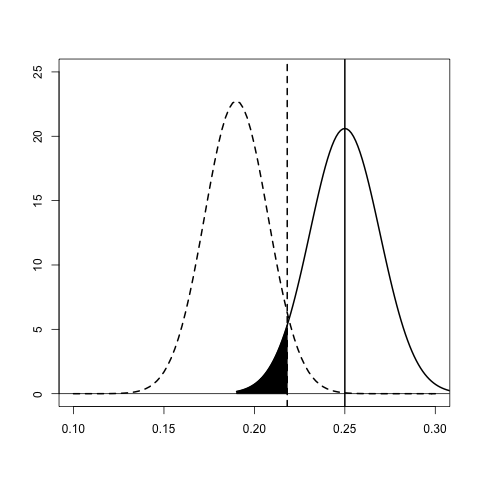
\includegraphics[width=12cm,height=6cm]{img/secEspConcurent}
\end{center}



\item Parmi une infinité d'estimations possibles de la proportion $p^\star=19\%$, on s'intéresse à la proportion de celles qui conduiront à ne pas accepter l'assertion d'intérêt du concurrent. Hachurez cette surface sur le graphique précédent. Quelle est l'instruction \texttt{R} permettant de l'obtenir~? Mathématiquement cette quantité est notée $\beta(19\%)$.



\item Cette surface est évaluée à 5.43\%. Que peut-on dire de $\beta(p)$ pour $p\leq 19\%$~? Si vous faites confiance en l'a priori du concurrent, lui conseillez-vous d'acheter l'échantillon de taille $n=500$~?



\item Le concurrent décide d'acheter l'échantillon, noté $\Vect{y}$, sur lequel 96 personnes (i.e. $19.2\%$) ont prétendu acheter le produit~A. Peut-on plutôt penser que moins de 25\% des clients du concurrent achèteront le produit~A ~? (indication : pas de rédaction standard, appliquez simplement la règle de décision)



\item On s'intéresse maintenant à l'estimation par intervalle de confiance du paramètre $p^A$. Proposez l'instruction \texttt{R} ayant permis d'obtenir le résultat ci-dessous correspondant à un intervalle de confiance au niveau de confiance de 90\% de $p^A$ calculé à partir du jeu de données $\Vect{y}$ que l'on note \texttt{y} en \texttt{R}~ (cet intervalle est noté $[\Int{p^A}{inf}{y} , \Int{p^A}{sup}{y} ]$:

\IndicR
\begin{Verbatim}[frame=leftline,fontfamily=tt,fontshape=n,numbers=left]
> # IC <- (instruction R à fournir dans la rédaction)
> IC
[1] 0.1630267 0.2209733
\end{Verbatim}




\item Le produit~A a été lancé sur le marché, et il a été alors possible d'évaluer le vrai paramètre $p^A$ à $18.9\%$. Pour essayer de faire comprendre à l'un de ses collègues comment il faut interpréter les intervalles de confiance (en particulier le précédent), le concurrent propose l'exercice pédagogique suivant. On construit une urne de taille $N=2000000$ boules dont une proportion $p^A=18.9\%$ sont numérotées 1 (les autres étant numérotées 0). On fait alors $199$ tirages de 500 boules au hasard au sein de cette urne. Les jeux de données créés sont donc de la même nature que $\Vect{y}$. Les $m=200$ jeux de données sont notés $\Vect{y_{[1]}}$, $\Vect{y_{[2]}}$, \ldots, $\Vect{y_{[200]}}$ (le premier $\Vect{y_{[1]}}$ correspondant à $\Vect{y}$). Pour chacun de ces jeux de données, on construit un intervalle de confiance au niveau de 90\% du paramètre $p^A$. 
Voici dans l'ordre des tirages quelques uns de ces intervalles~:


\begin{Verbatim}[frame=leftline,fontfamily=tt,fontshape=n,numbers=left]
pInf      pSup
  [1,] 0.1630267 0.2209733
  [2,] 0.1971384 0.2588616
  [3,] 0.2210000 0.2210000
...
[198,] 0.1649122 0.2230878
[199,] 0.1724662 0.2315338
[200,] 0.1573773 0.2146227
\end{Verbatim}


Parmi les $m=200$ intervalles de confiance, 179 contiennent le vrai paramètre $p^A$, qu'en pensez-vous~? Si l'on construisait une infinité d'intervalles de confiance, combien contiendraient le vrai paramètre $p^A$~?



\item Complétez sans justification les encadrés ci-dessous~: 

\begin{eqnarray}
\Prob{ \Int{p^A}{inf}{y_{[1]}} < p^A < \Int{p^A}{sup}{y_{[1]}} } &=&  \fbox{ \phantom{\textbf{\huge pastis}}} \nonumber \\
\Prob{ \Int{p^A}{inf}{y_{[2]}} < p^A < \Int{p^A}{sup}{y_{[2]}} } &=&  \fbox{ \phantom{\textbf{\huge pastis}}} \nonumber \\ 
\Prob{ \Int{p^A}{inf}{Y} < p^A < \Int{p^A}{sup}{Y} } &\simeq&  \fbox{ \phantom{\textbf{\huge pastis}}} \nonumber
\end{eqnarray}

\item Complétez sans justification les encadrés ci-dessous~:
\begin{list}{$\bullet$}{}
\item si le niveau de confiance avait été de 95\% alors
$$\Prob{ \Int{p^A}{inf}{y_{[1]}} < p^A < \Int{p^A}{sup}{y_{[1]}} } =  \fbox{ \phantom{\textbf{\huge pastis}}} $$
\item si le niveau de confiance avait été de 80\% alors
$$\Prob{ \Int{p^A}{inf}{y_{[2]}} < p^A < \Int{p^A}{sup}{y_{[2]}} } =  \fbox{ \phantom{\textbf{\huge pastis}}} $$
\end{list}
\item Complétez sans justification les encadrés ci-dessous~:
\begin{list}{$\bullet$}{}
\item si le niveau de confiance avait été de 95\% alors
$$\Prob{ \Int{p^A}{inf}{y_{[2]}} < p^A < \Int{p^A}{sup}{y_{[2]}} } =  \fbox{ \phantom{\textbf{\huge pastis}}} $$
\item si le niveau de confiance avait été de 80\% alors
$$\Prob{ \Int{p^A}{inf}{y_{[1]}} < p^A < \Int{p^A}{sup}{y_{[1]}} } =  \fbox{ \phantom{\textbf{\huge pastis}}} $$
\end{list}
\end{enumerate}
\end{exercice}






\end{document}


